\documentclass[../main]{subfiles}
\begin{document}
\chapter{Electroimanes}
\img{images/03/electroiman}{Electroimán compuesto por una batería, un
clavo y alambre de cobre esmaltado.}
\info{Fuerza de un eletroimán}{
  \begin{equation*}
    F=  40000\times B^2 \times s
  \end{equation*}

  \begin{equation*}
    F= \frac{ B^2 \times s}{2 \times \mu}
  \end{equation*}

  siendo:

  $F$: Fuerza producida por un eletroimán en kilopondios o kilogramos
  fuerza. $[Kp]$

  $B$: Inducción electromagnética en Tesla. $[T]$

  $S$: Sección de contacto en metros cuadrados. $[m^2]$

  $\mu$: Permeabilidad absoluta. $[\frac{T\times m}{ Av}]$

}
\actividad{Resolver los siguientes problemas.}

\begin{enumerate}
  \item El electroimán de la figura tiene aire entre el núcleo y la
    armadura \emph{entrehierro} una inducción magnética de $B=0,4T$.
    Calcular la fuerza de atracción del electroimán $F$.
    \begin{center}
      \begin{tikzpicture}[scale=0.8]
        \draw [stealth-stealth] (0,3)--(1,3) node[label=60]{};
        \draw [stealth-stealth] (4,3)--(3,4) node[label={right:60}]{};
        \draw [ultra thick] (0,0) --(-1,1);
        \draw [ultra thick] (0,0) --(0,1);
        \draw [ultra thick] (0,0) --(5,0)--(5,1)--(0,1);
        \draw [ultra thick] (0,1.2) --(0,6)--(5,6)--(5,1.2);
        \draw [ultra thick] (0,6) --(-1,7)--(4,7)--(5,6);
        \draw [ultra thick] (-1,7)
        --(-1,2.2)--(0,1.2)--(1,1.2)--(1,5)--(4,5)--(4,1.2)--(5,1.2);
        \draw [ultra thick] (-1,1)--(-1,2)--(0,1);
        \draw [ultra thick] (4,1.2)--(3,2.2)--(3,5);
        \draw [ultra thick] (1,2)--(3.2,2);
        \draw [ultra thick] (-1,2)--(-0.8,2);
        \draw [ultra thick] (5,1)--(4.8,1.2);
        \draw [thin] (1,5)--(1,6)--(0,7);
        \draw [thin,- Circle] (0,7)--(0,8);
        \draw [thin] (1.5,5)--(1.5,6)--(0.5,7);
        \draw [thin] (2,5)--(2,6)--(1,7);
        \draw [thin] (2.5,5)--(2.5,6)--(1.5,7);
        \draw [thin] (3,5)--(3,6)--(2,7);
        \draw [thin] (3.5,5)--(3.5,6)--(2.5,7);
        \draw [- Circle] (3,7)--(3,8);
      \end{tikzpicture}
    \end{center}
    %\img{images/03/1}{Problema 1}
  \item Calcular la fuerza con la que el electroimán de superficie de
    atracción de $S=96cm^2$ atraerá a su armadura si la inducción
    magnética en el hierro es de $B=500Gs$.
  \item El circuito magnético de la figura está construido de
    fundición de hierro y en el \emph{entrehierro} se desea una
    inducción magnética $B=1T$. Calcular el valor de la intensidad de
    la corriente $I$, que debe circular por la bobina de $N=1000$
    espiras considerando que ningún flujo se dispersa fuera del circuito.
    \begin{center}
      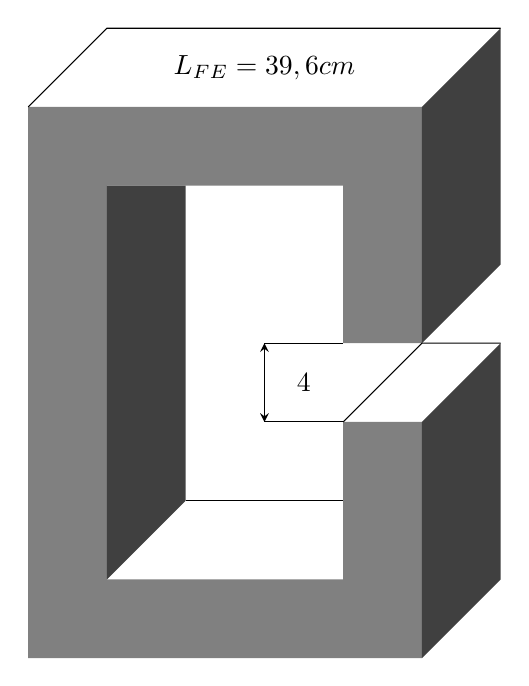
\begin{tikzpicture}
        \path
        [fill=gray](0,0)--(5,0)--(5,3)--(4,3)--(4,1)--(1,1)--(1,6)--(4,6)--(4,4)--(5,4)--(5,7)--(0,7)--(0,0);
        \path  [fill=darkgray](5,0)--(6,1)--(6,4)--(5,3)--(5,0);
        \path  [fill=darkgray](5,4)--(6,5)--(6,8)--(5,7)--(5,4);
        \path  [fill=darkgray](1,1)--(2,2)--(2,6)--(1,6)--(1,1);
        \draw (2,2)--(4,2);
        \draw (0,7)--(1,8)--(6,8);
        \draw (4,3)--(5,4)--(6,4);
        \draw (3,3)--(4,3);
        \draw (3,4)--(4,4);
        \draw [stealth-stealth] (3,3)--(3,4);
        \draw (3.5,3.5) node[]{$4$};
        \draw (3,7.5) node[]{$L_{FE}=39,6cm$};
      \end{tikzpicture}
    \end{center}
    %\img{images/03/3}{Problema 3}
  \item El anillo cilíndrico de la figura de sección $S=5cm^2$ está
    construido de chapa magnética, se desea un flujo de $\Phi
    =75000Mx$. Calcular la inducción magnética en el núcleo, longitud
    de la línea media y amperios -vuelta necesarios.
    \begin{center}
      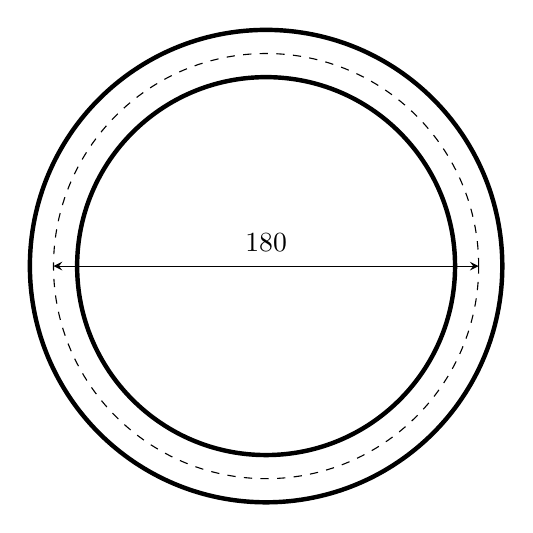
\begin{tikzpicture}[scale=0.03]
        \draw [dashed, thin] (0,0) circle [radius=90];
        \draw [ultra thick] (0,0) circle [radius=100];
        \draw [ultra thick] (0,0) circle [radius=80];
        \draw [stealth-stealth] (-90,0)--(90,0);
        \draw (0,10) node[]{180};
      \end{tikzpicture}
    \end{center}
    %\img{images/03/4}{Problema 4}
  \item El circuito de la figura está construido de chapa magnética,
    se desea una inducción de $B=1,8T$. Calcular la intensidad de
    campo $H$ en el hierro, longitud de la línea media,
    amperios-vuelta necesarios, intensidad que circula por la bobina
    de $N=200$ espiras.
    \begin{center}
      \begin{tikzpicture}[scale=0.03]
        \draw [ultra thick] (0,0) rectangle (180,180);
        \draw [ultra thick] (40,40) rectangle (140,140);
        \draw [thin,dashed] (20,20) rectangle (160,160);
        \draw [thin,Circle -] (-20,140)--(40,140);
        \draw [thin] (0,130)--(40,130);
        \draw [thin] (0,120)--(40,120);
        \draw [thin] (0,110)--(40,110);
        \draw [thin] (0,100)--(40,100);
        \draw [thin] (0,90)--(40,90);
        \draw [thin] (0,80)--(40,80);
        \draw [thin] (0,70)--(40,70);
        \draw [thin] (0,60)--(40,60);
        \draw [thin] (0,50)--(40,50);
        \draw [thin,Circle -] (-20,40)--(0,40);
        \draw [stealth-stealth] (140,80)--(180,80);
        \draw [stealth-stealth] (40,100)--(140,100);
        \draw [stealth-stealth] (100,140)--(100,40);
        \draw [stealth-stealth] (80,40)--(80,0);
        \draw (80,110) node[]{100};
        \draw (110,70) node[]{100};
        \draw (170,90) node[]{40};
        \draw (70,30) node[]{40};
      \end{tikzpicture}
    \end{center}
    %\img{images/03/5}{Problema 5}
  \item El circuito de la figura formado por chapa magnética está
    sometido a una inducción magnética de $B=15000Gs$. Calcular
    intensidad de campo magnético $H$ en la chapa magnética, longitud
    de la línea media, intensidad de campo magnético en el aire,
    amperio-vuelta totales, número de espiras $N$ de la bobina para
    que la intensidad sea de $I=4A$.
    \begin{center}
      \begin{tikzpicture}
        \draw [ultra thick]
        (4,0)--(4,1)--(1,1)--(1,3)--(3,3)--(3,1.2)--(4,1.2)--(4,4)--(0,4)--(0,0)--(4,0);
        \draw [thin,dashed] (0.5,0.5) rectangle (3.5,3.5);
        \draw [stealth-stealth] (0,-1)--(0.5,-1)-- node[]{20}(0.5,-1)--(1,-1)  ;
        \draw [stealth-] (1,-1)--(2,-1) node[]{40} [-stealth](2,-1)--(3,-1);
        \draw [stealth-stealth] (3,-1)--(3.5,-1) --node[]{20} (3.5,-1)--(4,-1);
        \draw [stealth-stealth] (5,4)--(5,3) node[label={right:20}]{} ;
        \draw [stealth-] (5,3)--(5,2.2) node[label={right:30}]{};
        \draw [-stealth] (5,2.2)--(5,1.2);
        \draw [stealth-stealth] (4,1.2)--(4,1) node[label={right:2}]{};
        \draw [stealth-stealth] (5,1)--(5,0) node[label={right:20}]{};
        \draw [thin,Circle -] (-1,3)--(0,3)--(1,2.5);
        \draw [thin] (0,2.5)--(1,2);
        \draw [thin] (0,2)--(1,1.5);
        \draw [thin] (0,1.5)--(1,1);
        \draw [thin,Circle -] (-1,1)--(0,1);
        \draw [thin] (0,0)--(0,-1);
        \draw [thin] (1,0)--(1,-1);
        \draw [thin] (3,0)--(3,-1);
        \draw [thin] (4,0)--(4,-1);
      \end{tikzpicture}
    \end{center}
    %\img{images/03/6}{Problema 6}
\end{enumerate}
\end{document}

